
\input macro3
\usepackage{fullpage,amsmath,amssymb,amsthm}

\newcommand{\D}{\displaystyle}

\title{Math 199 CD3 Merit Worksheet 16: Review for Upcoming Midterm}
\date{\today}


\begin{document}

\maketitle

\section{Hydrostatic Force}

Find the hydrostatic force on the following plates submerged in water as shown in each image. In each case consider the top of the shaded “box” to be the surface of the water in which the plate is submerged. Note as well that the dimensions in many of the images will not be perfectly to scale in order to better fit the plate in the image. The lengths given in each image are in meters.
\begin{enumerate}
	\item Image:
	\newline
			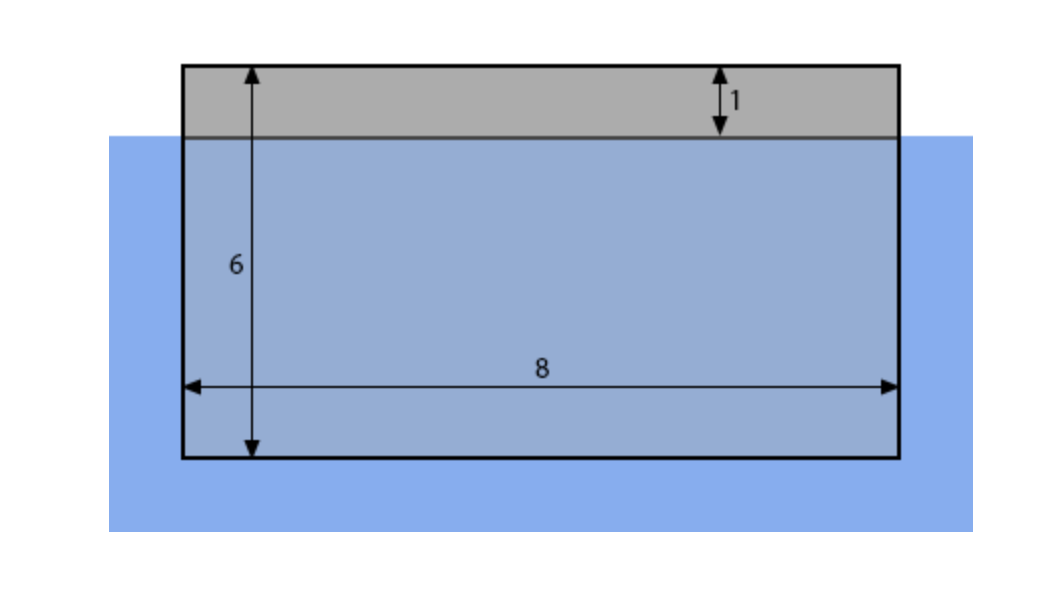
\includegraphics[scale=0.7]{1.png}	
			\vfill
			\newpage
	\item Image:
	\newline
			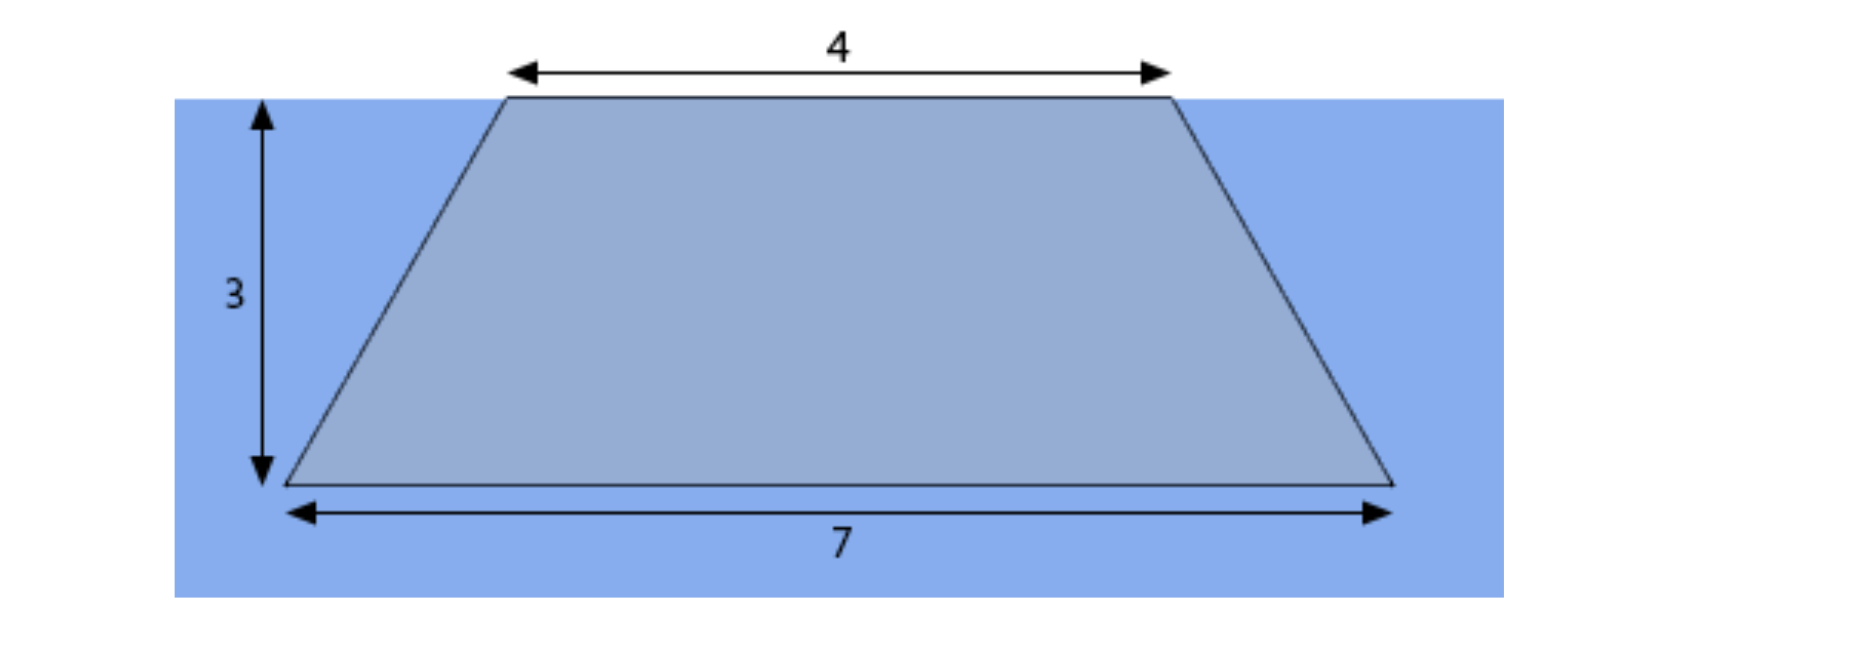
\includegraphics[scale=0.3]{2.png}	
\vfill
	\item Image:
	\newline
			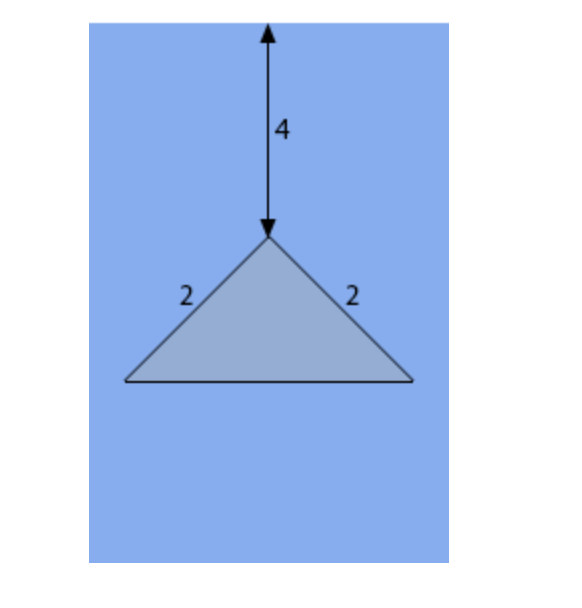
\includegraphics[scale=0.7]{3.png}
			\vfill
			\newpage
\section{Centroid}
\item Please state the formula for moments and center of mass before attempt any of the below problems
\vfill 
\item Determine the center of mass of the region bounded by $y=2\sin(2x)$, $y=0$ on the interval $[0, \pi/2]$
\vfill 
\item Determine the center of mass of the region bounded by $y=x^3$ and $y=\sqrt x$	
\vfill
\newpage
\section{Series}
Everything up to absolutely convergence and conditionally convergence should be on the exam, please study them. 
\subsection{These problems should just be routine, please try to do all of them}
Determine whether the following series converge or diverge. NOte that it is not always possible to use alternating series test. After you decided the series diverge or converge, pick your favorite numer $n$ and calculate the error up to its first $n$ terms if possible (some expression might be too hard to integrate then you can skip). Please state any inequality you are going to use for estimating, but more importantly, tell me what it means

 	\item $$\sum_0^\infty (-1)^n\frac{n+1}{2n+1}$$
 	\vfill
 	\item Estimate the error by its first 10 terms, 
 	$$\sum_1^\infty\frac{(-1)^{n+1}}{n^2}$$
 \vfill
 \item $$\sum_0^\infty\frac{n!}{(2n)!}$$

 \vfill
 \item $$\sum_1^\infty n(3/4)^n$$
 \vfill
 \newpage
 \item Study this series 
 $$1-\frac{2^2+1}{2^3+1}+\frac{3^2+1}{3^3+1}+\cdots$$
 \vfill
 \item $$\sum_1^\infty\frac{n^3}{(\ln2)^n}$$
 \vfill
 \item  $$\sum_1^\infty\frac{n^3}{(\ln3)^n}$$
 \vfill
\newpage
\item
 $$\sum \frac{x^n}{n!}$$
    \vfill
    \item
    $$\sum n!x^n$$
    \vfill 
    \item 
    $$\sum \frac{2}{3+5n}$$
    \vfill

    \item
    $$\sum \frac{n^2}{n^3+1}$$
    \vfill
    \newpage
 \subsection{Conditionally convergence}
 Determine if the series converge conditionally or absolutely, using both alternating series test or LCT
 \item $$\sum_1^\infty \frac{(-1)^{n+1}}{\sqrt{n+1}+\sqrt{n}}$$
\vfill
\item $$\sum_1^\infty (-1)^{n+1}\frac{n^2}{e^n}$$
]\vfill


\end{enumerate}
\end{document}